\documentclass{report}
\usepackage{cours}

\linespread{1.2}

\title{Optimization of simplified calculation methods for early age cracking assessment}
\author{Edgar Pierre BURKHART}
\date{2020}

\bibliography{bib}

\begin{document}

\maketitle

\tableofcontents
%%%


\chapter{Literrature review}

\section{Introduction}

Cracking control is a critical point in the design of concrete structures.
Uncontrolled cracking can have a major impact on the durability of reinforced
concrete structures, for several reasons including corrosion of metal rods.
For this reason, the risks of cracking during the early age of a structure have
been studied by numerous research teams in the past. In this chapter, the
results that have been found regarding the evaluation of cracking risks will be
observed.

\section{Creep, Shrinkage and Cracking of Restrained Concrete at Early Age
\cite{cscea}}
\subsection{Introduction}
In 2001, a research team from the University of Illinois realised an
experimental study of the impact of creep and shrinkage on cracking of
restrained concrete regarding various parameters.

\subsection{Methods}
An experimental study was conducted using a uniaxial restrained shrinkage test.
A combination of restrained and unrestrained specimens was used to extract
creep from the results. According to the authors, the difference in strain
between free shrinkage and restrained tests was the creep strain, as seen in
\autoref{aci1}. The experiment's goal was to determine a number of properties
of concrete at early age.

This study was conducted with both normal and high performance concrete as
well as plain and fiber reinforced concrete. The aggregates used were always
the same, and both steel fibers and polypropylene fibers were used in fiber
reinforced concrete. The impact of water to concrete ratio was studied, at
static temperature and humidity values, with two different drying environements
being used.

\begin{figure}
  \centering
  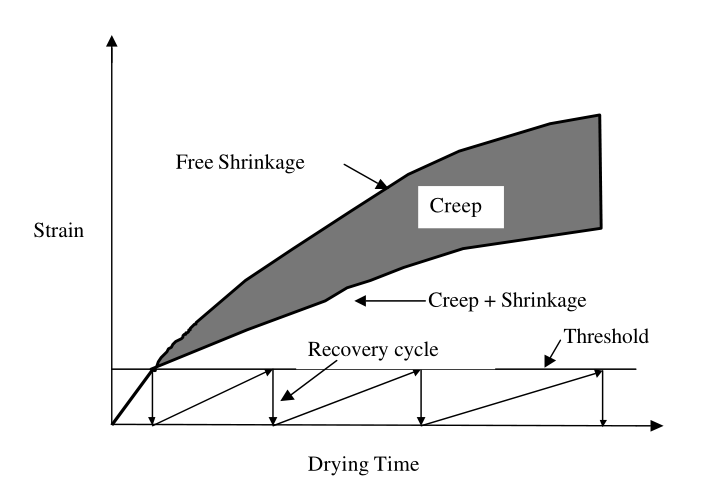
\includegraphics[width=.5\linewidth]{fig/aci1}
  \caption{Schematic diagram of the test mechanism \cite{cscea}.}\label{aci1}
\end{figure}

\subsection{Results}
According to the free shrinkage study, a first stage in which no shrinkage is
experienced by the concrete seems to occur, which is supposed to be caused by
evaporative cooling of the concrete specimens leading to a slight expansion of
the specimens. In the first 10 hours of the study, expansion or shrinkage could
occur depending on the sample.

The results also display a high shrinkage rate during the following 40 hours of
testing. The study of fiber-reinforced concrete showed that steel fibers did
not impact shrinkage, while the use of polypropylene fibers led to a small
increase of free shrinkage.

Although all restrained shrinkage specimens cracked, fracturing time varied
strongly among the different specimens. A lower rate of shrinage was observed
for higher water to concrete ratio, causing longer fracturing times. Steel
fiber reinforced specimens also showed delayed fracturing for all water to
concrete ratios, with more higher delays for low water to concrete ratios. By
contrast, polypropylene fibers caused earlier failure due to the shrinkage
behavior observed before.

According to the findings of this study, other factors than tensile stress have
an importance in cracking behavior of restrained concrete. For instance,
high-performance concrete cracked earlier than normal concrete despite
sustaining the same tensile stress. Stress history has a strong influence on
the performance of the material regarding cracking. Other findings include that
the failing stress is not equal to the tensile strength of the material, and is
lower by around \SIrange{20}{25}{\percent}.

%%%
\printbibliography
\end{document}
